% RNN / sequence prediction section (MNIST-Rows)
% Intended insertion point: after the MNIST experiments section.

\section{Sequence prediction on MNIST-Rows}\label{sec:mnist_rows_rnn}

We evaluate whether TeReL can be extended to a simple recurrent setting under a locality constraint. The task is \texttt{mnist-rows}: given an image row sequence, the model predicts the next row in a one-step autoregressive objective ($x_t \rightarrow x_{t+1}$). We report validation one-step prediction mean squared error (MSE).

As a baseline, we compare against a backpropagation-trained recurrent model optimized with backpropagation through time (BPTT).

\subsection{Quantitative results}
We additionally report the per-timestep latent update magnitude $\lVert \Delta h \rVert_2 = \lVert h_t - h_{t-1} \rVert_2$ as a coarse summary of state dynamics. In this setup, TeReL yields larger step-to-step state changes than the backpropagation baseline (Table~\ref{tab:mnist_rows_one_step}), consistent with a more dynamic hidden-state trajectory over the sequence.

\begin{table}[h!]
  \centering
  \caption{One-step next-row prediction on \texttt{mnist-rows} (20 epochs). Lower MSE is better.}
  \begin{tabular}{lccc}
    \toprule
    \textbf{Model} & \textbf{Val.\ one-step MSE} & $\mathbf{\mu(\lVert \Delta h \rVert_2)}$ & $\mathbf{\sigma(\lVert \Delta h \rVert_2)}$ \\
    \midrule
    TeReL local-state + concat\_mlp & 0.22345 & 5.62 & 4.28 \\
    BP RNN baseline (MLP)        & 0.17569 & 4.06 & 2.80 \\
    \bottomrule
  \end{tabular}
  \label{tab:mnist_rows_one_step}
\end{table}

The TeReL sequence variant achieves substantially lower loss than earlier TeReL-RNN baselines in this project and serves as our primary TeReL sequence result; however, the backpropagation baseline remains better on pure one-step prediction loss.

In this section, we focus on one-step prediction as the primary evaluation target rather than long-horizon generation. We include multi-step autoregressive rollouts in the appendix to illustrate qualitative sequence prediction behavior.

Additional experimental details and qualitative rollouts are provided in Appendix~\ref{app:rnn-details}.

Additional experimental details and qualitative rollouts are provided in Appendix~\ref{app:rnn-details}.

\subsection{Latent trajectory visualization}
To compare the learned sequence dynamics, we visualize per-timestep latents with t-SNE and summarize mean latent trajectories across timesteps. Each TeReL plot is placed side-by-side with the corresponding backpropagation baseline plot for direct visual comparison.

\begin{figure}[!ht]
  \centering
  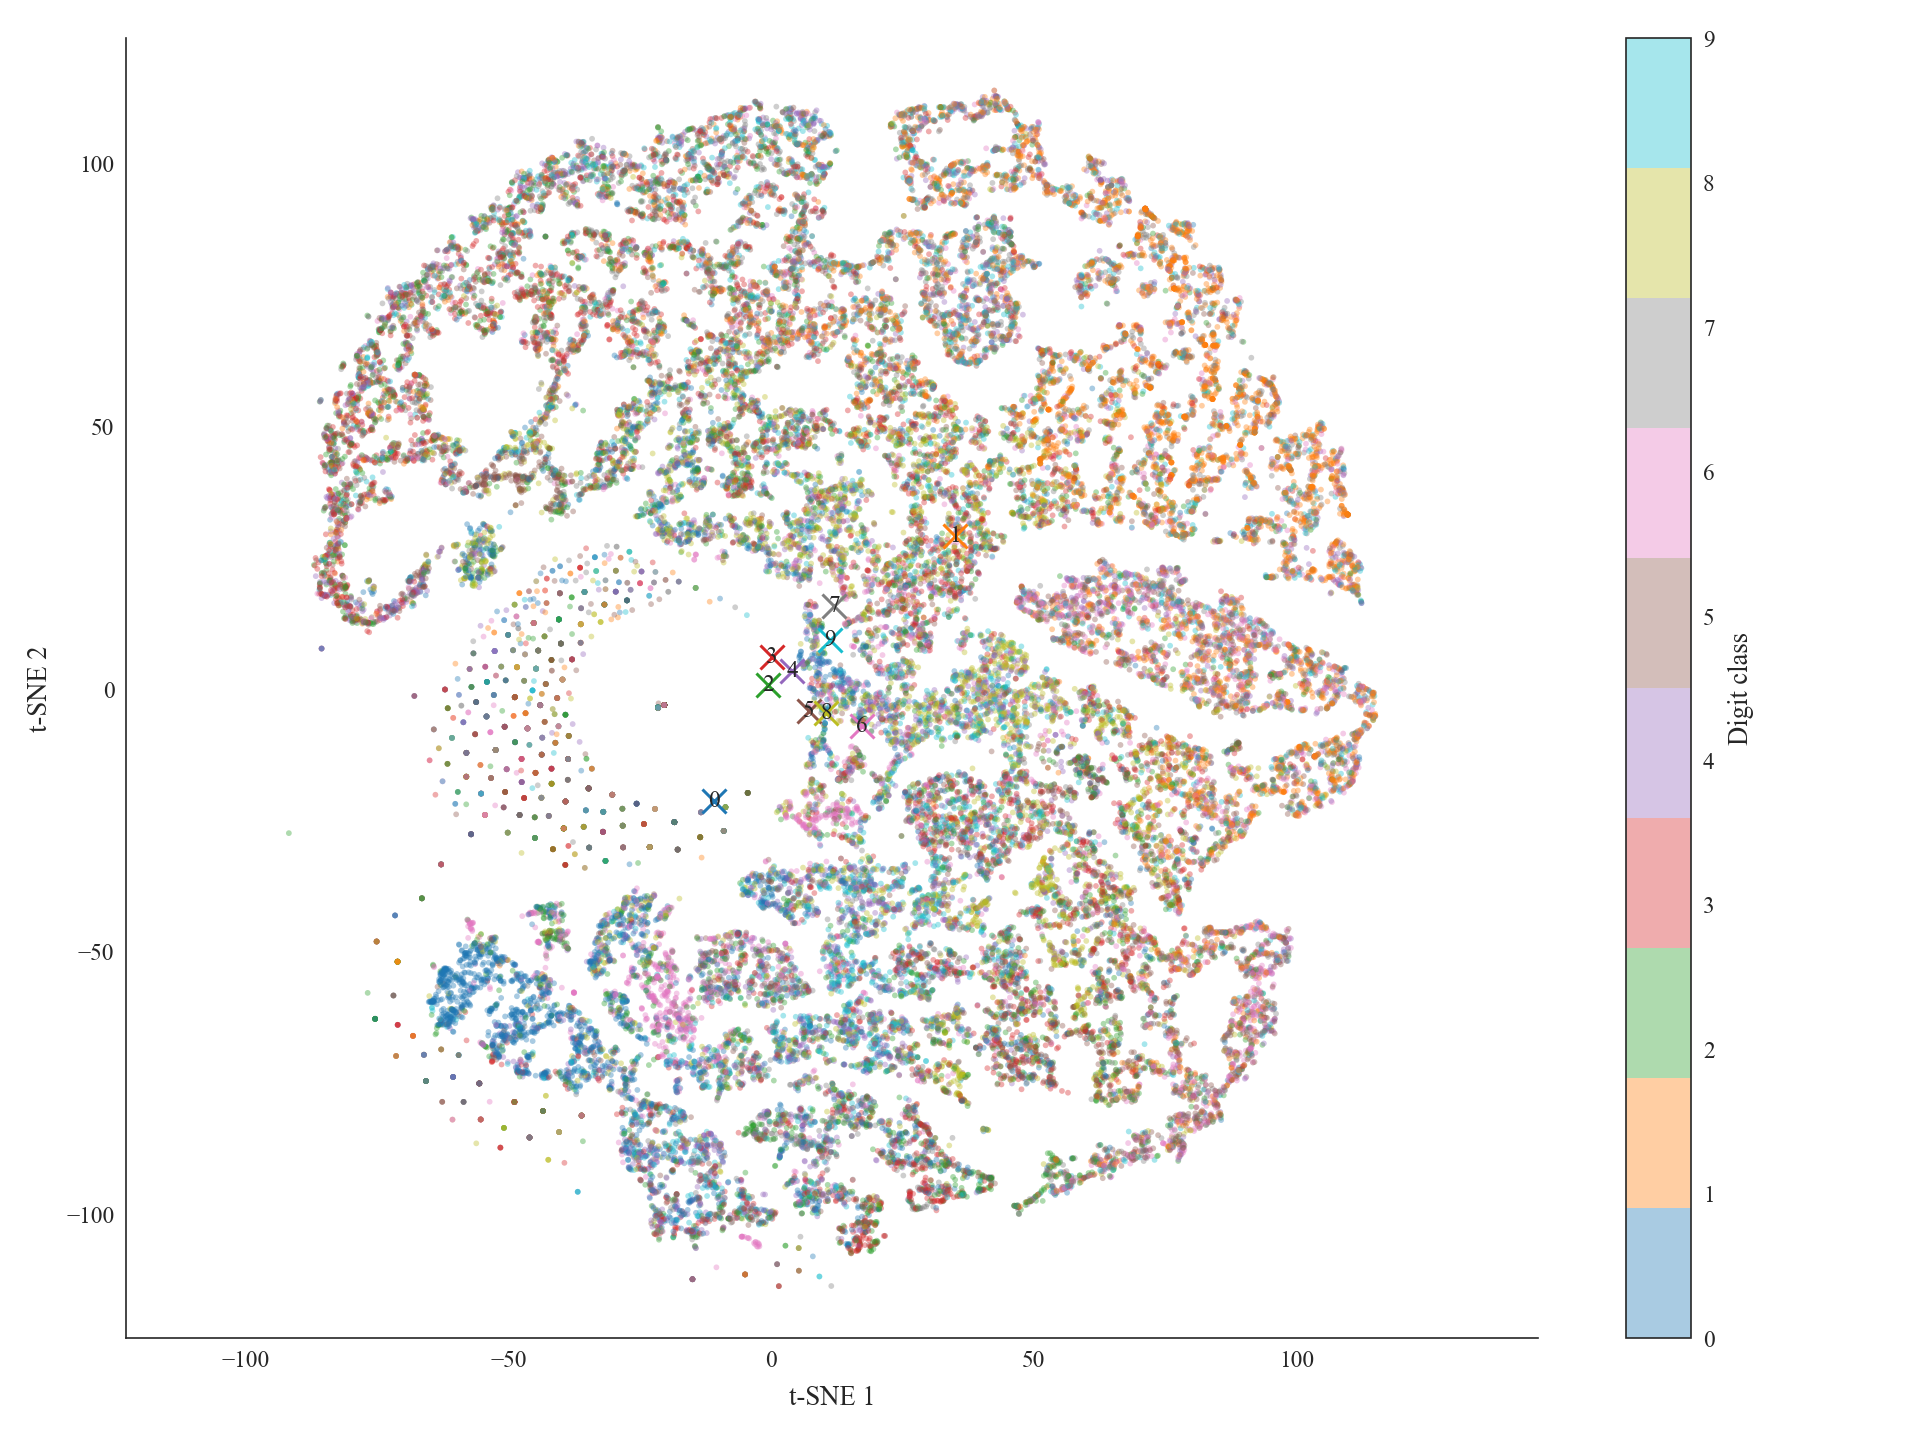
\includegraphics[width=0.49\linewidth]{terel_rnn_20ep/sequence_latent_tsne_samples.png}
  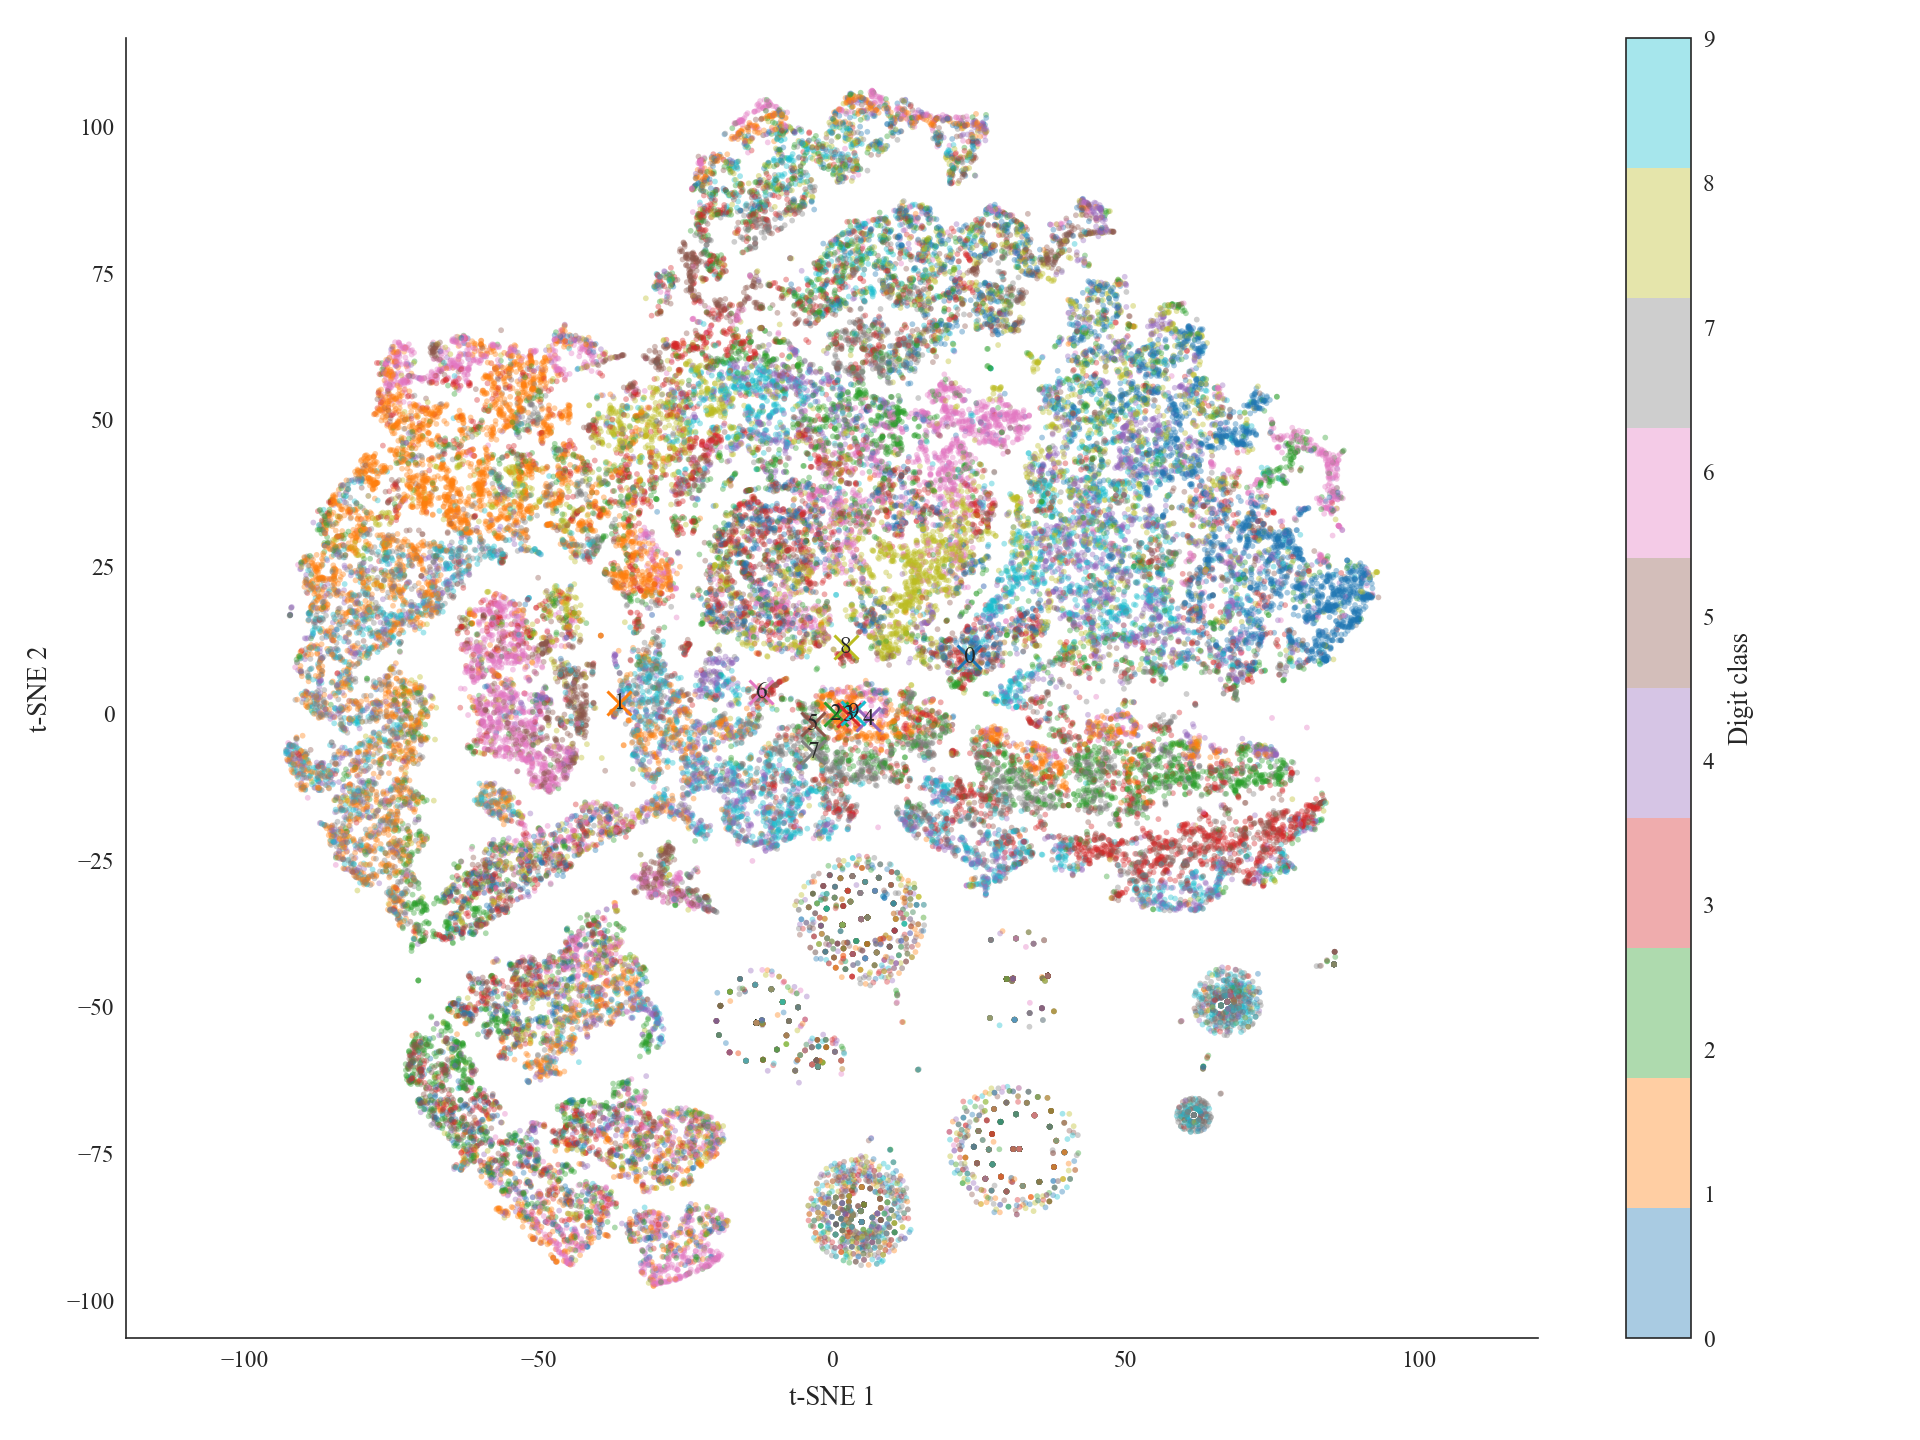
\includegraphics[width=0.49\linewidth]{bp_rnn_mnist_rows/sequence_latent_tsne_samples.png}
  \caption{t-SNE projection of per-timestep sequence latents. \textbf{Left:} TeReL. \textbf{Right:} BP.}
  \label{fig:mnist_rows_tsne_samples}
\end{figure}
\FloatBarrier

\begin{figure}[!ht]
  \centering
  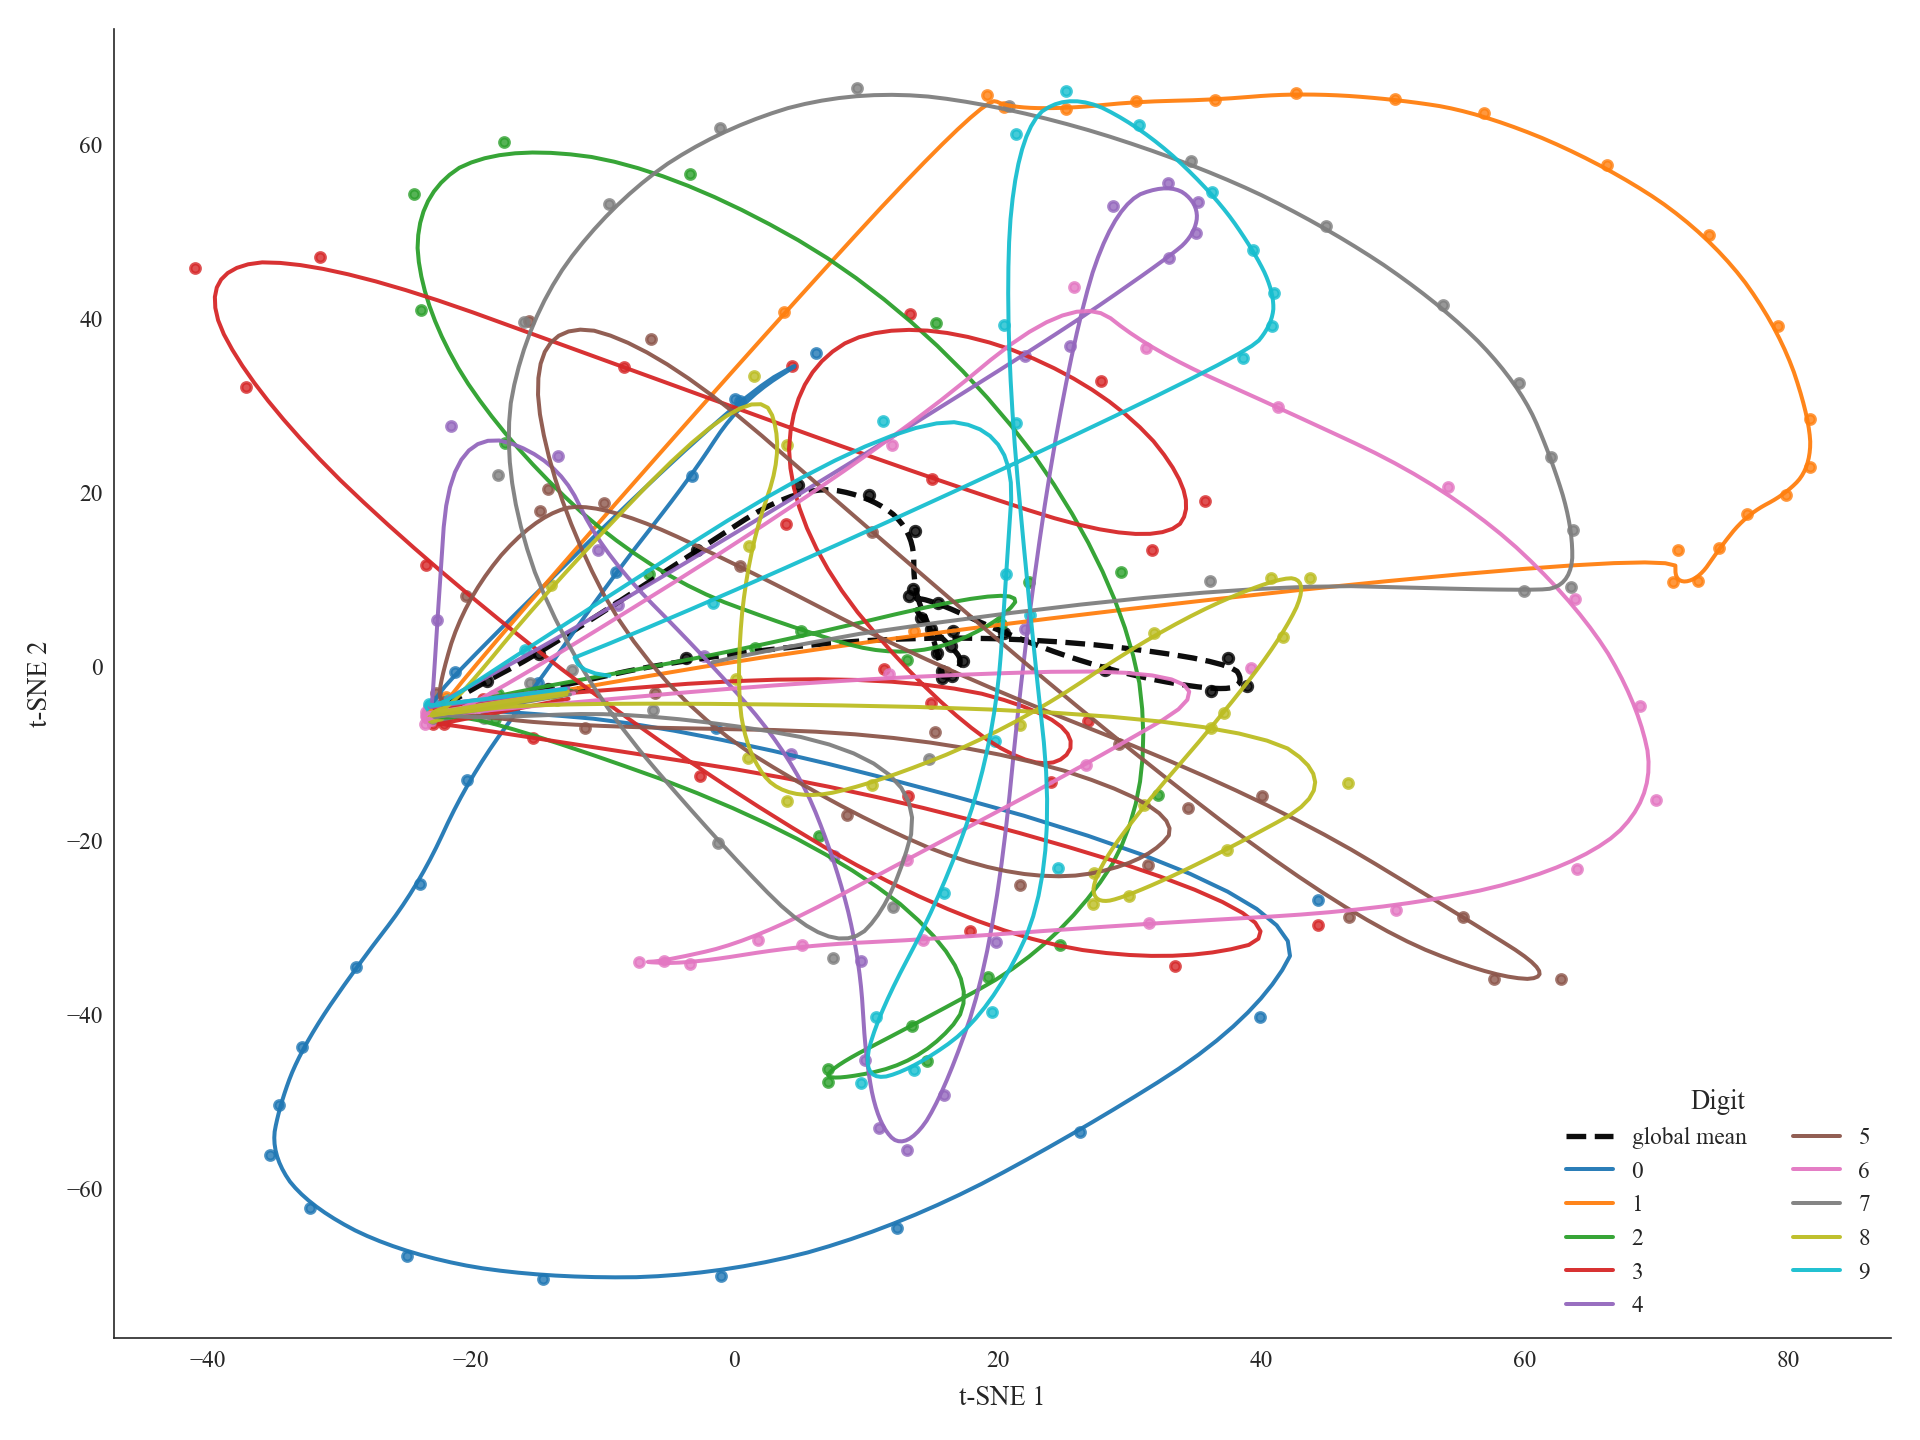
\includegraphics[width=0.49\linewidth]{terel_rnn_20ep/sequence_latent_tsne_mean_paths.png}
  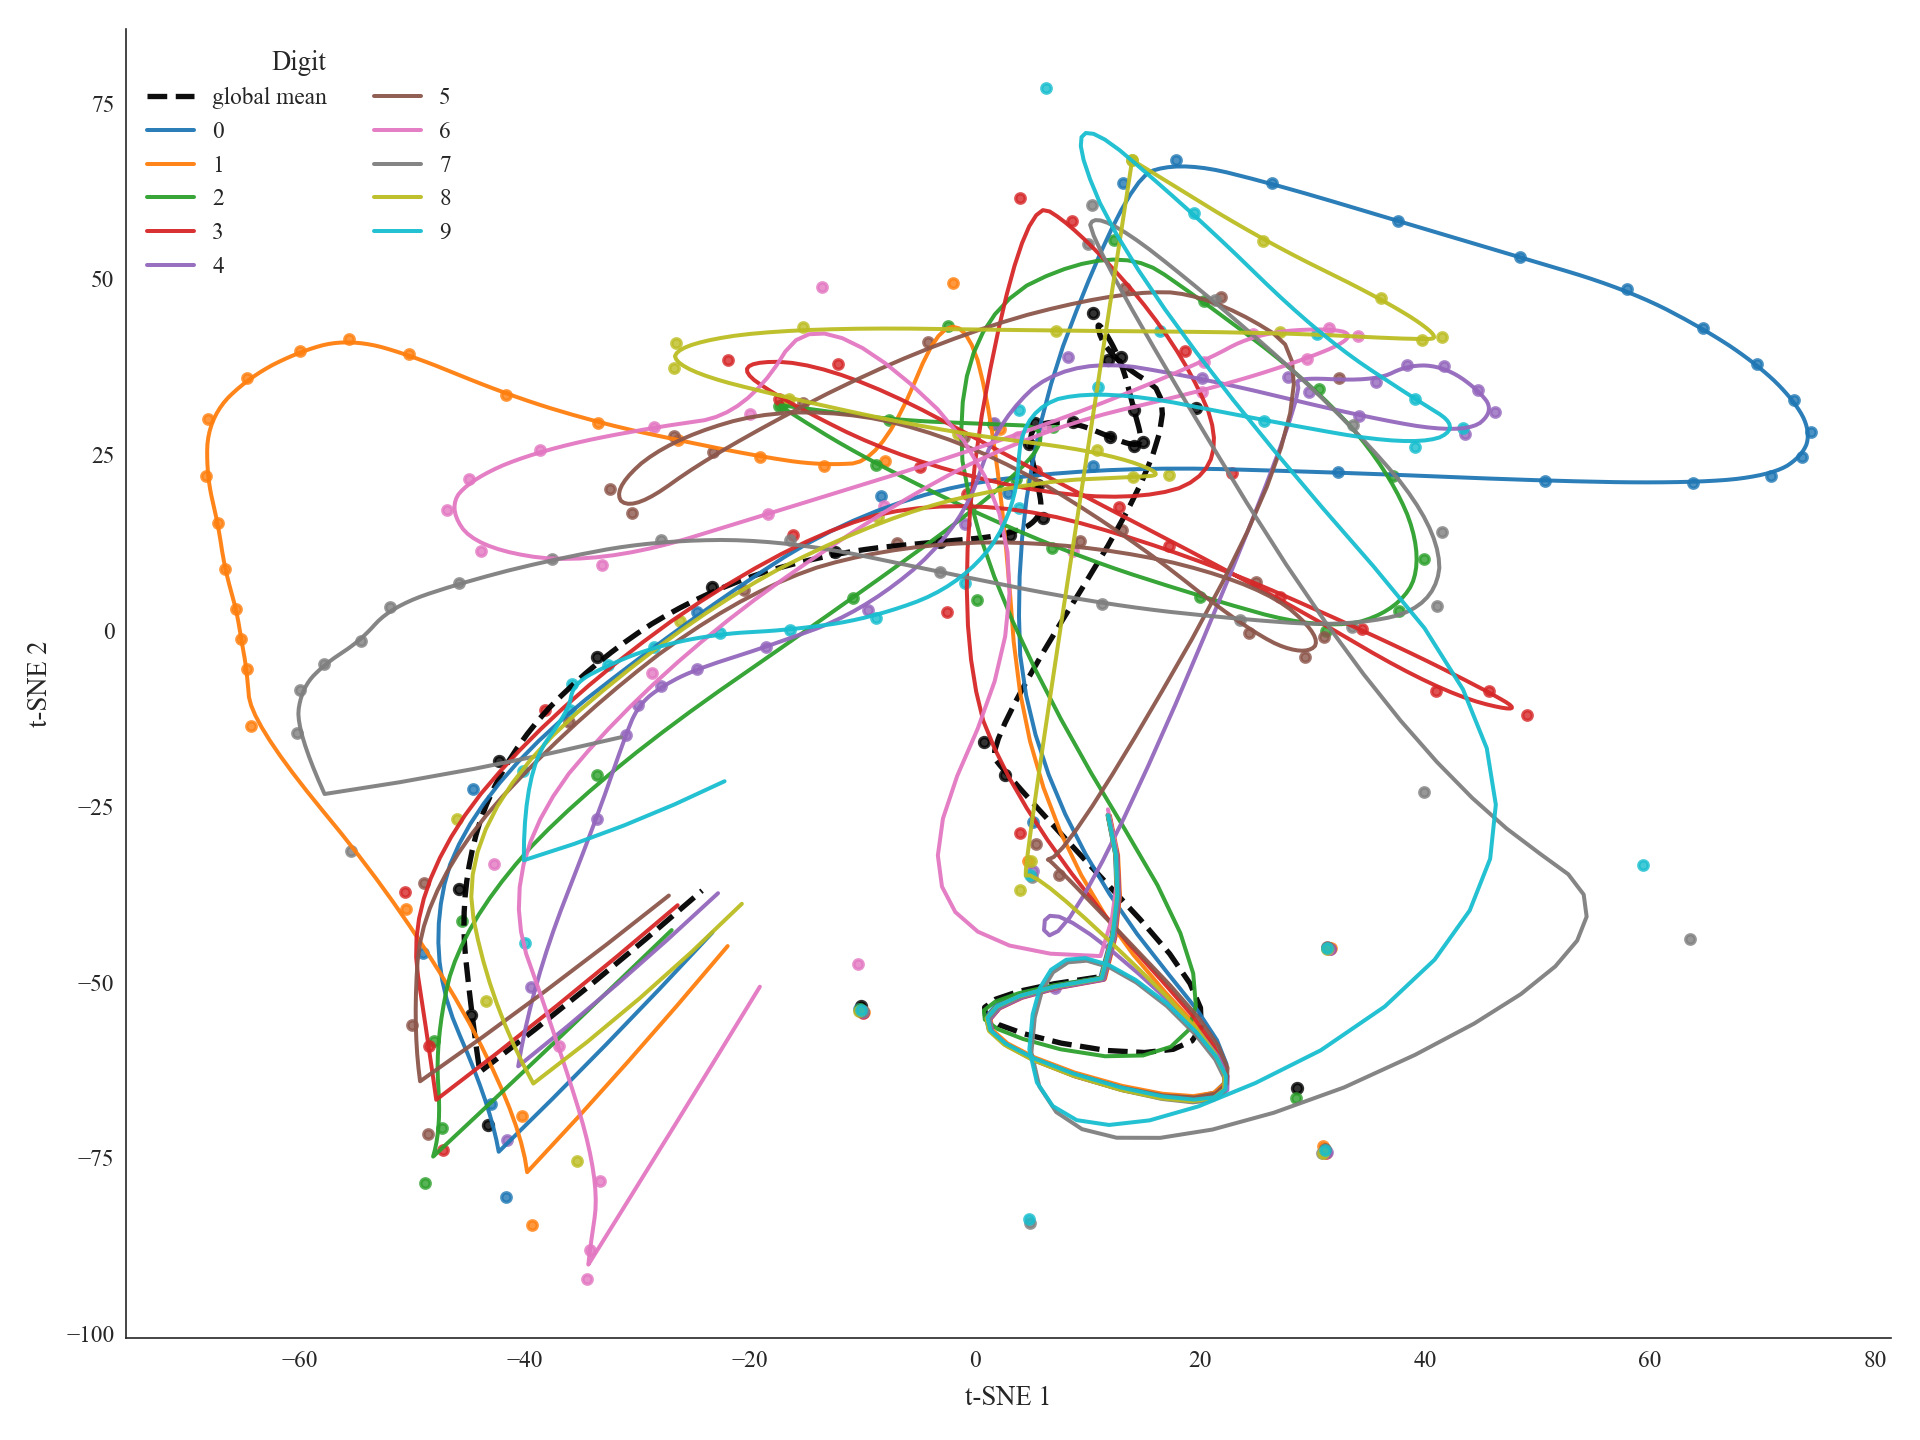
\includegraphics[width=0.49\linewidth]{bp_rnn_mnist_rows/sequence_latent_tsne_mean_paths.png}
  \caption{Smoothed mean trajectories in t-SNE space: a global mean path across all samples and a class-mean path per digit. \textbf{Left:} TeReL. \textbf{Right:} BP.}
  \label{fig:mnist_rows_tsne_mean_paths}
\end{figure}
\FloatBarrier

\begin{figure}[!ht]
  \centering
  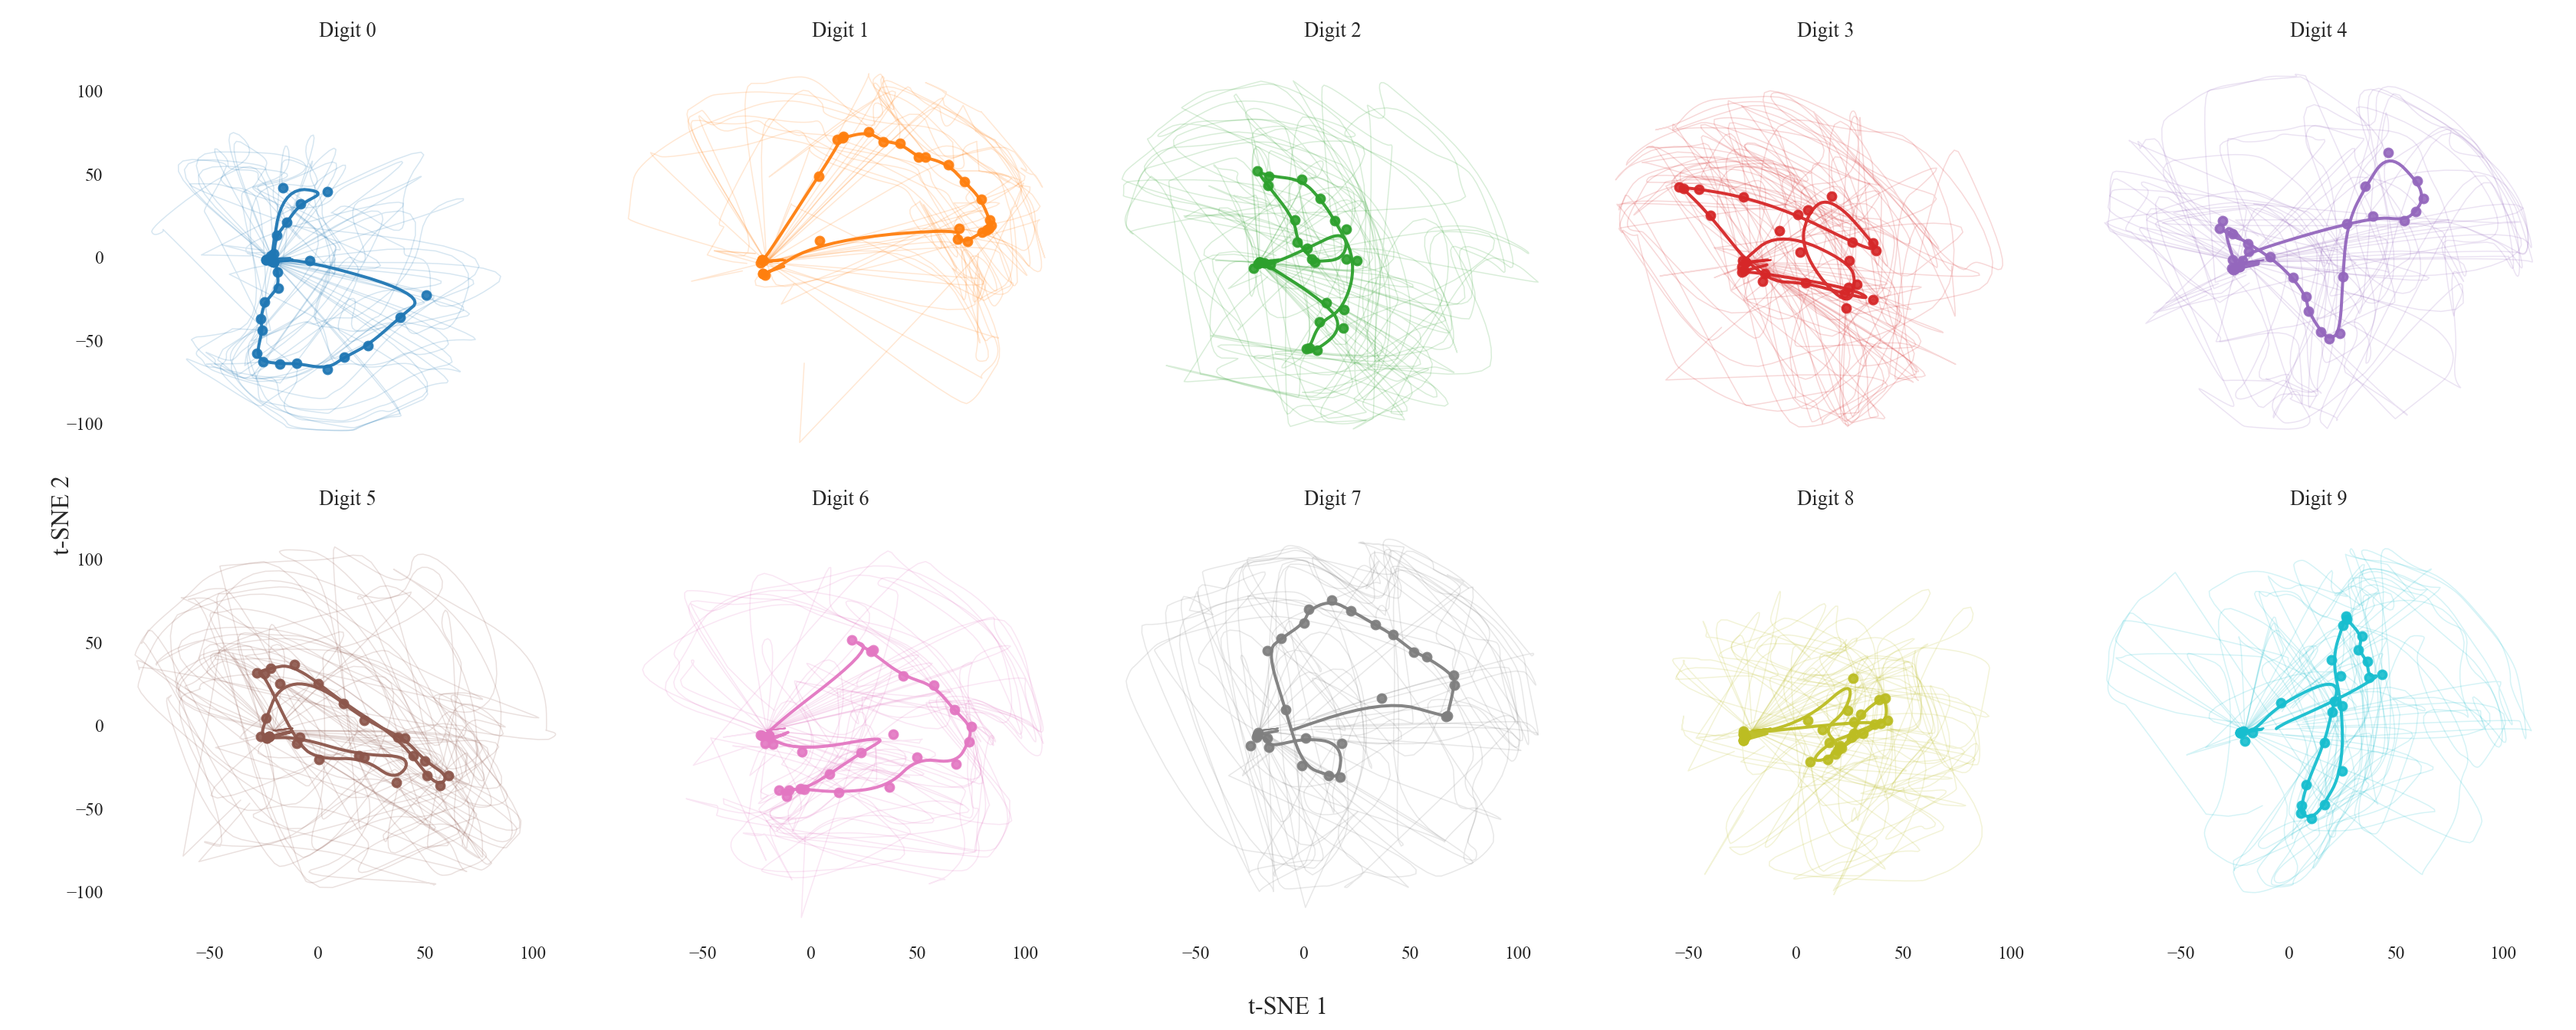
\includegraphics[width=0.49\linewidth]{terel_rnn_20ep/sequence_latent_tsne_per_digit_paths.png}
  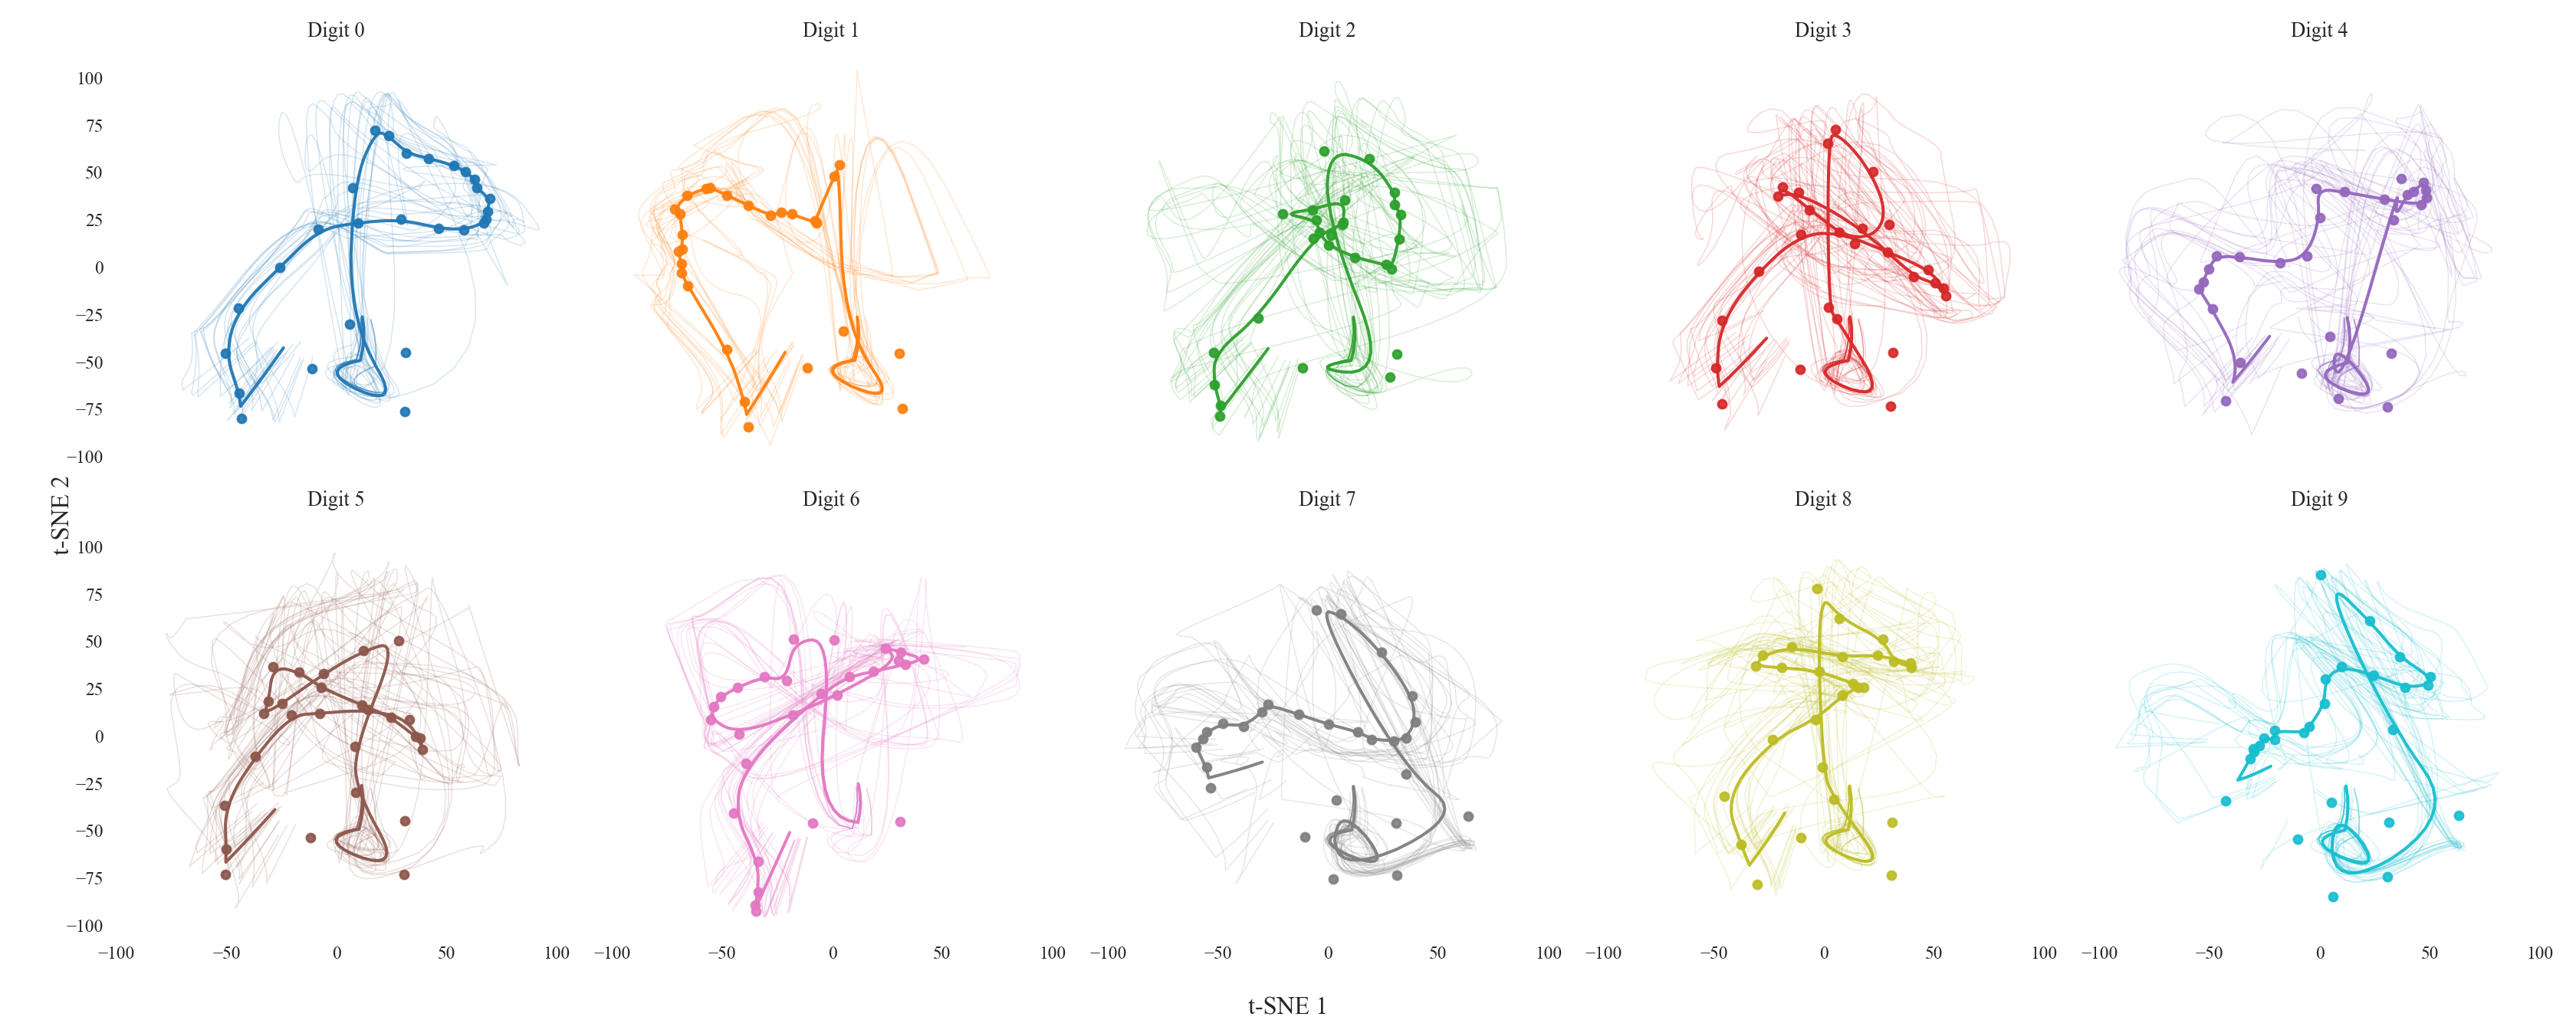
\includegraphics[width=0.49\linewidth]{bp_rnn_mnist_rows/sequence_latent_tsne_per_digit_paths.png}
  \caption{Per-digit trajectory panels in t-SNE space. Each panel shows smoothed sample paths for one digit together with the digit mean path and timestep markers. \textbf{Left:} TeReL. \textbf{Right:} BP.}
  \label{fig:mnist_rows_tsne_per_digit_paths}
\end{figure}
\FloatBarrier

\noindent In this space, both models learn digit-specific progression paths with partial class separability, suggesting a learned row-progression manifold. Qualitatively, TeReL shows particularly clear per-digit structure for digits 0, 1, and 9, while the backpropagation baseline shows this most strongly for digits 2, 4, and 6. While TeReL mean trajectories are more identifiable, backpropagation produces more coherent hidden-state progressions.

\subsection{Architecture details and the role of preprocessing}
Our architecture consists of a preprocessor, a recurrent aggregator, and a linear prediction head. In the TeReL model, we impose the constraint that no backpropagation, including backpropagation through time (BPTT), is performed, preserving an online-compatible update rule.

The model is split into (i) a per-timestep preprocessor that maps the raw row $x_t$ to features $y_t$, (ii) a recurrent aggregator that fuses $(y_t, h_{t-1})$ into a new state $h_t$, and (iii) a linear head that predicts the next row $x_{t+1}$ from $h_t$. In our TeReL sequence model, both the preprocessor and the recurrent aggregator are trained using the TeReL objective, while the linear head is trained for the next-row prediction task.

In our experiments, using a standard RNN-style aggregator directly on raw rows without a preprocessor did not yield meaningful performance. We attribute this to a distribution mismatch between the raw input rows and the evolving hidden state, which makes direct fusion of $(x_t, h_{t-1})$ brittle. Introducing a preprocessor trained with a TeReL objective alleviates this mismatch, since both inputs are represented by a vector optimized under the TeReL-objective.
